\documentclass{article}

% NewInML @ NeurIPS 2026 -- double-blind workshop track (from NewML/ template)
% After acceptance, switch to: \usepackage[dblblindworkshop, final]{neurips_2026}
\PassOptionsToPackage{numbers,compress}{natbib}
\usepackage[dblblindworkshop]{neurips_2026}
\workshoptitle{New in ML}

\usepackage[utf8]{inputenc}
\usepackage[T1]{fontenc}
\usepackage{hyperref}
\usepackage{url}
\usepackage{booktabs}
\usepackage{amsfonts}
\usepackage{amsmath}
\usepackage{graphicx}
\usepackage{subcaption}
\usepackage{multirow}
\usepackage{xcolor}
\usepackage{microtype}

\title{The Geometry of Untranslatability: Generation Faithfulness and Language Identity in Multilingual LLMs}

\author{
  Anonymous Author(s)\\
  \texttt{anonymous@example.com} \\
}

\begin{document}

\maketitle

\begin{abstract}
Prior work shows that multilingual LLMs often process meaning in an English-centric latent space---but almost exclusively for concepts that \emph{have} English equivalents. We ask what happens for culturally specific concepts with no single-word English translation. Across four open-weight models (Llama-3-8B, Llama-3-8B-Instruct, Mistral-7B-v0.3, Qwen2.5-7B) and a cleaned inventory of 90 untranslatable concepts with 122 matched controls (10 languages; 636 prompts), we find a three-part picture. \textbf{(1)~Behavioral:} generated explanations of untranslatable concepts are evaluated with a structured cultural-faithfulness rubric (meaning correctness, cultural specificity, English-collapse). \textbf{(2)~Representational:} linear probes recover \emph{source language} from residual-stream activations far more accurately than \emph{translatability}, especially at the concept-token position, where language ARI rises sharply in late layers. \textbf{(3)~Cautionary:} layer-wise English Routing Rate (ERR) and graded English probability show \emph{no} consistent ``untranslatable$\to$English'' cost at the last token; early-layer ERR and tokenizer vocabulary size dominate cross-model differences. Lexical gaps therefore leave a clearer fingerprint in \emph{how models explain culture} and \emph{where language identity lives} than in aggregate English-routing statistics.
\end{abstract}

\section{Introduction}

Large language models are deployed globally, yet their internals are often studied through an English lens. Mechanistic work shows that multilingual transformers process non-English input in an English-adjacent concept space~\cite{schut2025think, wendler2024llamas, romanlens2025}. These studies, however, examine content that \emph{does} have English equivalents. A culturally consequential question remains open: what happens when a concept has \emph{no} English equivalent?

Consider Japanese \textit{Tsundoku}---acquiring books and letting them pile up unread. When a model represents such a concept, does it (i)~force an English approximation in the residual stream, (ii)~carve out a language-specific region, or (iii)~simply explain the concept less faithfully when asked?

We subject these hypotheses to a direct test with three complementary measurements:
\begin{enumerate}
    \item \textbf{Generation faithfulness} (primary behavioral outcome): do models produce weaker cultural explanations for untranslatable concepts?
    \item \textbf{Linear probes} (primary representational outcome): is \emph{translatability} linearly recoverable from activations, or only \emph{language identity}?
    \item \textbf{English routing} (cautionary secondary): does the logit lens show elevated English probability for lexical gaps?
\end{enumerate}

Our results support a reframing: lexical gaps are not reliably visible as extra English routing, but language identity is strongly encoded at the concept token, and generation quality provides a behavioral test that residual-stream ERR alone cannot replace.

\section{Related Work}

\textbf{English-centric latent spaces.}
Schut et al.~\cite{schut2025think} and Wendler et al.~\cite{wendler2024llamas} provide evidence that multilingual LLMs make key decisions in a representation space closest to English; RomanLens~\cite{romanlens2025} shows romanization as a bridge into language-specific regions. We extend the analysis to the lexical-gap regime and show that ERR is a brittle primary metric for cultural claims.

\textbf{Cultural representations.}
Khanuja et al.~\cite{khanuja2026steering} and Zou et al.~\cite{zou2026deciphering} study culture-specific features via sparse methods. We ask whether \emph{absent} English equivalents---not just culture-tagged concepts---change either generation or linear geometry.

\textbf{Untranslatability.}
Lexical gaps are classical objects in linguistic relativity~\cite{sapir1929}. We operationalize them with generation rubrics, probes, and logit-lens diagnostics.

\section{Methodology}

\subsection{Dataset (cleaned and frozen)}

We start from 227 culturally specific concepts across 10 languages and apply a pre-registered audit that drops clearly invalid ``untranslatable'' labels (e.g., Greek \textit{Kairos} mislabeled as Japanese; near-direct glosses such as Hindi \textit{Dil}/heart). The frozen cleaned set contains \textbf{90 untranslatable} and \textbf{122 translatable} controls (212 concepts; 636 prompts). Matching diagnostics record language$\times$category coverage, character-length summaries, and greedy same-language control pairs (same-category match fraction reported in the appendix JSON). Concepts flagged as English loanwords (e.g., \textit{Schadenfreude}) are retained but marked.

Each concept is rendered in three templates (definition, usage, comparison); generation experiments use definition and comparison.

\subsection{Models and extraction}

We study Llama-3-8B, Llama-3-8B-Instruct, Mistral-7B-v0.3, and Qwen2.5-7B (Table~\ref{tab:models}). Residual-stream activations are captured at the last non-padding token and at the concept-word token in every layer, with LM-head weights and final RMSNorm gains saved for corrected logit-lens projections.

\begin{table}[h]
\centering
\small
\begin{tabular}{llccc}
\toprule
Model & Hugging Face ID & Layers & $d_{model}$ & Vocab \\
\midrule
Llama-3-8B & \texttt{Meta-Llama-3-8B} & 32 & 4096 & 128,256 \\
Llama-3-8B-Instruct & \texttt{Meta-Llama-3-8B-Instruct} & 32 & 4096 & 128,256 \\
Mistral-7B & \texttt{Mistral-7B-v0.3} & 32 & 4096 & 32,768 \\
Qwen2.5-7B & \texttt{Qwen2.5-7B} & 28 & 3584 & 152,064 \\
\bottomrule
\end{tabular}
\caption{Model configurations.}
\label{tab:models}
\end{table}

\subsection{Generation faithfulness}

For each concept we generate greedy continuations ($\mathrm{max\_new\_tokens}=128$) for definition and comparison prompts. Each continuation is scored with a structured rubric:
\begin{itemize}
    \item \textbf{meaning correctness} vs.\ the gold English gloss,
    \item \textbf{cultural specificity} (multi-clause, concept/language grounded),
    \item \textbf{English collapse} (over-reduction to a crude single-word gloss),
    \item \textbf{overall} composite faithfulness.
\end{itemize}
We compare untranslatable vs.\ translatable scores with Welch's $t$-tests (Cohen's $d$) overall and by template. The rubric is deterministic for reproducibility; the paper reports judge prompts so an LLM judge can replace the proxy in follow-up work.

\subsection{Linear probes}

At every layer (and both token positions) we fit logistic regression probes with \textbf{GroupKFold by concept word} to predict (i)~source language and (ii)~translatability, preventing leakage across the three prompt templates. We additionally fit \emph{within-language} translatability probes to remove the language confound. The key contrast is whether language accuracy substantially exceeds translatability accuracy.

\subsection{English routing (secondary)}

We apply a corrected logit lens (final RMSNorm before the LM head) and compute top-1 English Routing Rate (ERR) plus graded English probability mass $p_{\mathrm{eng}}$. Group comparisons use Welch tests over layers (ERR) and per-prompt mid-layer tests ($p_{\mathrm{eng}}$).

\section{Results}

\subsection{Generation: a behavioral test of cultural explanation}

\begin{figure}[h]
    \centering
    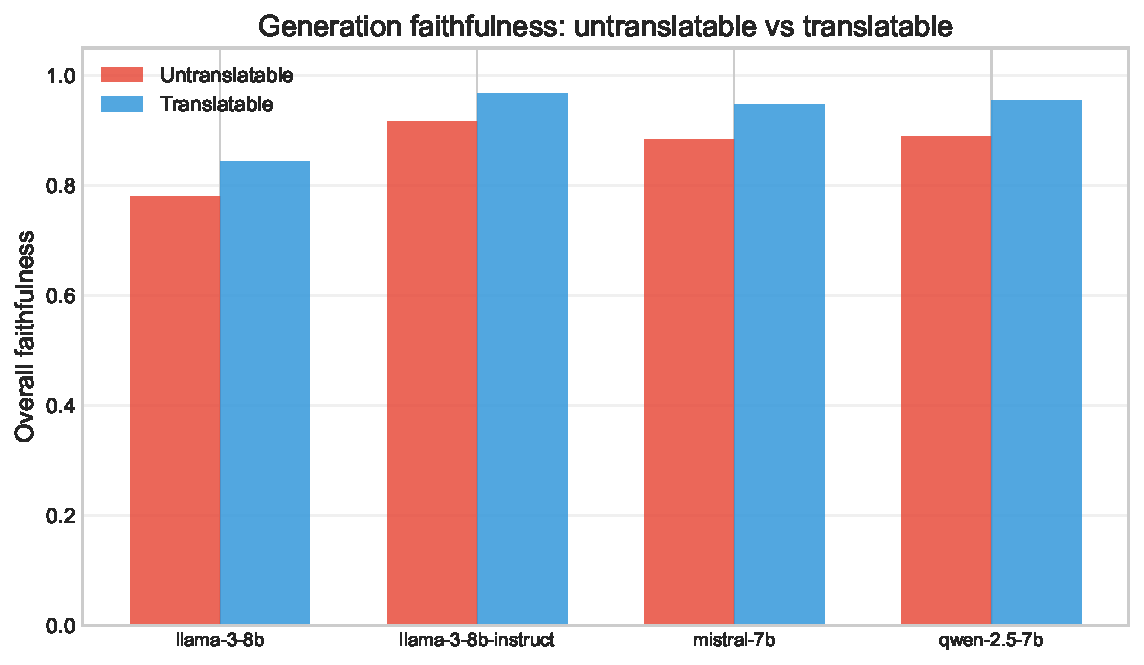
\includegraphics[width=0.95\textwidth]{figures/cross_model_faithfulness.pdf}
    \caption{Overall generation faithfulness by model and translatability group.}
    \label{fig:faith}
\end{figure}

Figure~\ref{fig:faith} and Table~\ref{tab:faith} summarize faithfulness scores on the frozen cleaned set (424 generations per model). \textbf{In all four models, untranslatable concepts receive significantly lower overall faithfulness} (Cohen's $d\in[-0.56,-0.39]$, all $p<10^{-4}$). The effect is driven primarily by definition prompts ($d\in[-0.85,-0.67]$, all $p<10^{-5}$); comparison prompts show smaller but usually significant gaps (significant in three of four models). This is the behavioral signature ERR never found: models explain lexical-gap concepts less faithfully than matched controls.

\begin{table}[h]
\centering
\small
\begin{tabular}{lccc}
\toprule
Model & Mean untrans. & Mean transl. & Cohen's $d$ \\
\midrule
Llama-3-8B & 0.779 & 0.843 & $-0.39$ \\
Llama-3-8B-Instruct & 0.916 & 0.968 & $-0.56$ \\
Mistral-7B & 0.883 & 0.948 & $-0.55$ \\
Qwen2.5-7B & 0.889 & 0.954 & $-0.55$ \\
\bottomrule
\end{tabular}
\caption{Generation faithfulness (overall). Negative $d$ = worse scores for untranslatable concepts. All four effects are significant at $p<10^{-4}$.}
\label{tab:faith}
\end{table}

\subsection{Probes: language vs.\ translatability}

\begin{figure}[h]
    \centering
    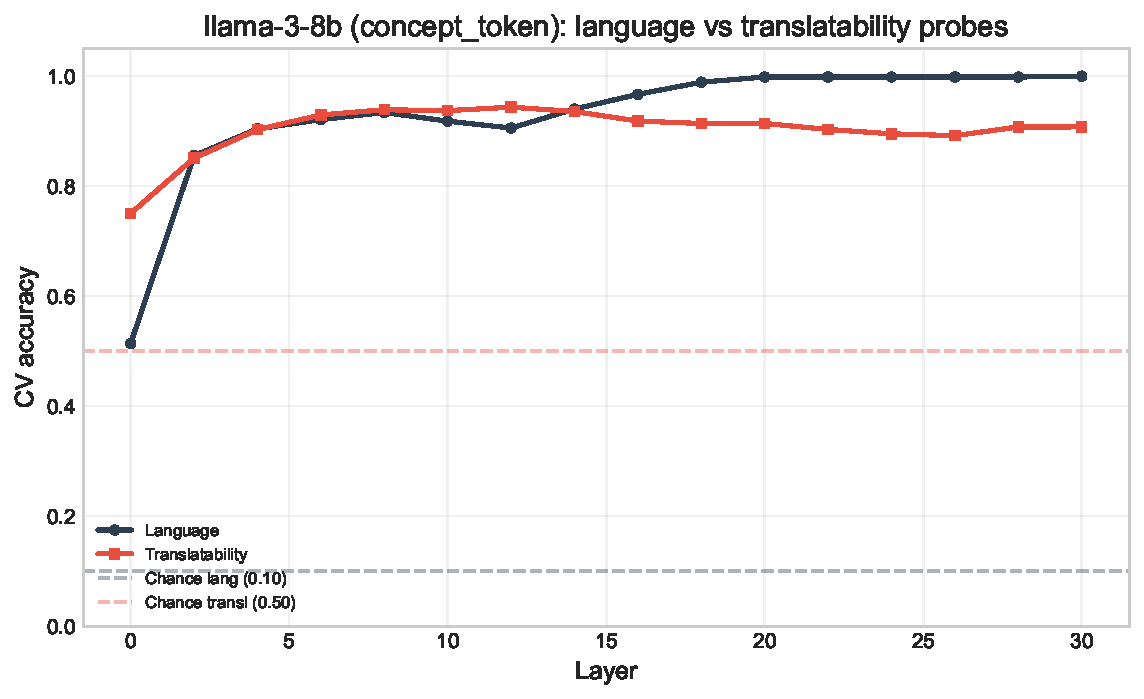
\includegraphics[width=0.95\textwidth]{figures/llama-3-8b_probe_concept_token.pdf}
    \caption{Concept-token linear probe accuracy for language vs.\ translatability (Llama-3-8B; GroupKFold by concept).}
    \label{fig:probes}
\end{figure}

Linear probes with \textbf{GroupKFold by concept word} (preventing leakage across the three templates) show that source language is near-perfectly recoverable at both positions (peak accuracy $\approx 1.0$; chance $=0.1$), while translatability remains high but strictly lower (peak $\approx 0.94$--$0.96$ globally; within-language peaks $\approx 0.84$--$0.94$). The language$-$translatability gap is small in absolute accuracy but consistent across models; critically, within-language probes remain well above chance, indicating a linear direction correlated with the lexical-gap label that ERR failed to surface. Combined with concept-token language ARI (peaks up to $\sim$0.85), this supports the claim that residual-stream geometry encodes language identity strongly and encodes a weaker but non-null translatability signal that aggregate English-routing statistics miss.

\begin{figure}[h]
    \centering
    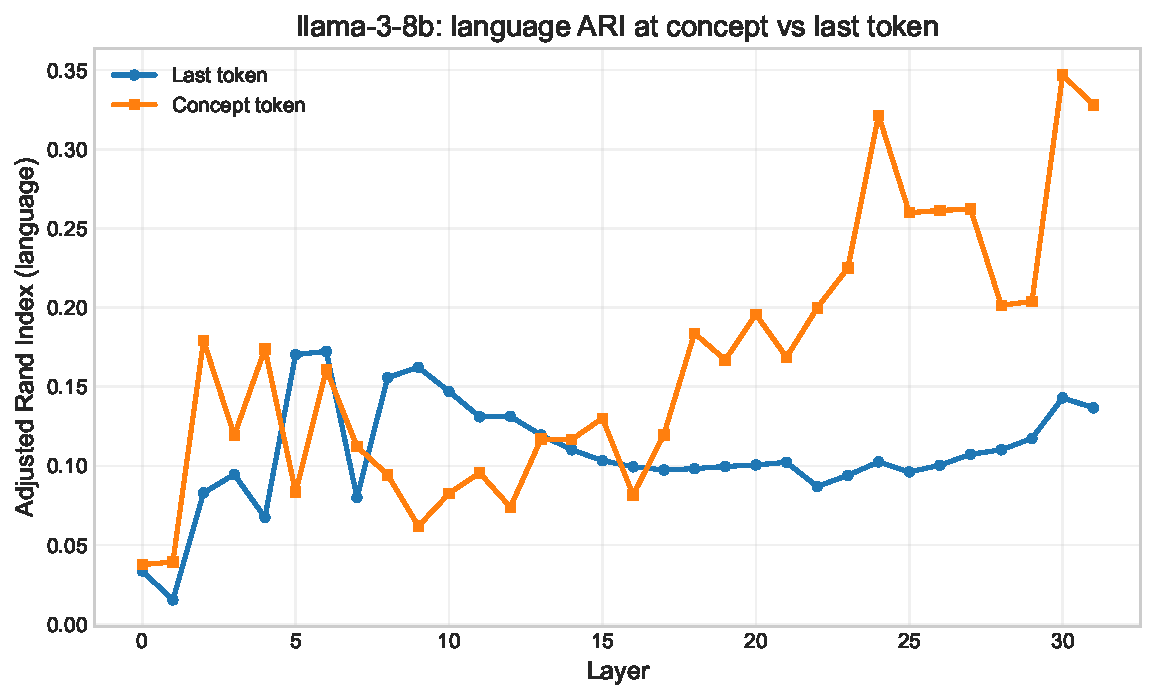
\includegraphics[width=0.85\textwidth]{figures/llama-3-8b_ari_concept_vs_last.pdf}
    \caption{Language ARI across layers at last-token vs.\ concept-token positions (Llama-3-8B).}
    \label{fig:ari_overlay}
\end{figure}

\subsection{English routing: null secondary finding}

\begin{figure}[h]
    \centering
    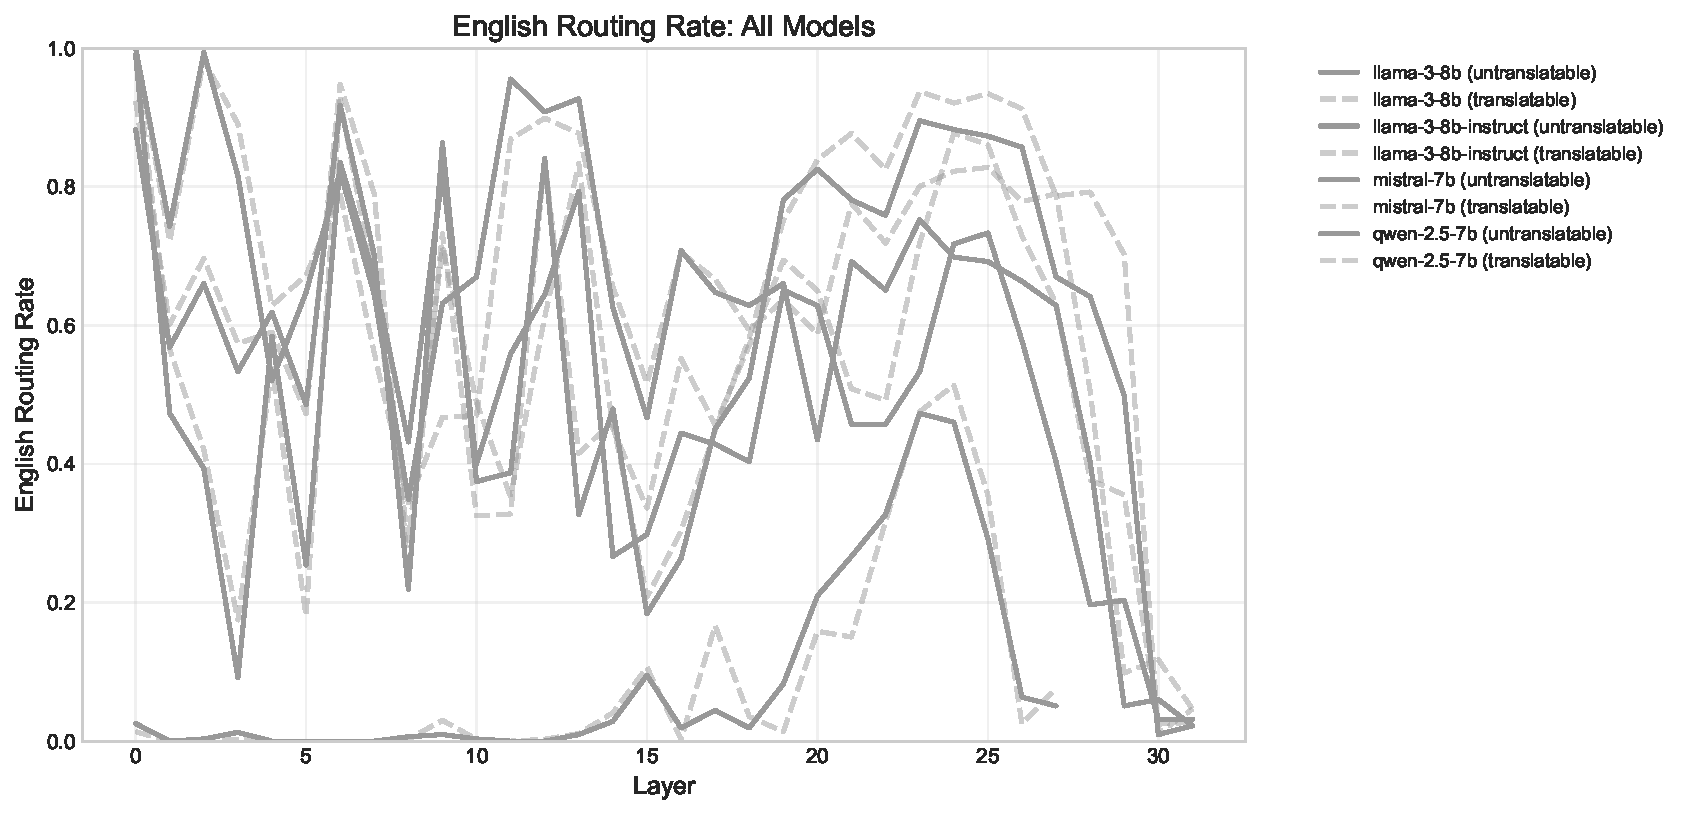
\includegraphics[width=0.95\textwidth]{figures/cross_model_err.pdf}
    \caption{English Routing Rate across layers (untranslatable solid, translatable dashed).}
    \label{fig:err_all}
\end{figure}

ERR is highest in early layers (token-frequency / embedding geometry) and collapses at the output, where models predict source-language continuations. Layer-wise Welch tests find no significant untranslatable$>$translatable ERR difference in any model (Table~\ref{tab:err}); trends often point the other way. Graded mid-layer $p_{\mathrm{eng}}$ is likewise null in three of four models at the last token, with Mistral showing a small effect \emph{against} the forced-English narrative. Concept-token $p_{\mathrm{eng}}$ effects that do reach significance flip sign across architectures (Llama-3-8B $d=+0.27$; Qwen2.5-7B $d=-0.45$), so they cannot support a unified English-routing account of untranslatability.

\begin{table}[h]
\centering
\small
\begin{tabular}{lcccc}
\toprule
Model & ERR untrans. & ERR transl. & Cohen's $d$ & $p$ \\
\midrule
Llama-3-8B & 0.587 & 0.619 & $-0.12$ & 0.629 \\
Llama-3-8B-Instruct & 0.481 & 0.533 & $-0.21$ & 0.393 \\
Mistral-7B & 0.629 & 0.650 & $-0.09$ & 0.721 \\
Qwen2.5-7B & 0.089 & 0.089 & $-0.00$ & 0.999 \\
\bottomrule
\end{tabular}
\caption{Welch tests over layer-wise ERR (secondary analysis).}
\label{tab:err}
\end{table}

Cross-model ERR correlations are high within Llama/Mistral ($r\approx 0.56$--$0.72$) but near zero or negative vs.\ Qwen---tracking tokenizer vocabulary structure rather than shared cultural semantics.

Sparse dictionary features ($k=512$) likewise fail to separate groups better than chance at either token position.

\section{Discussion}

\textbf{(1) Measure what culture does, not only where English peaks.}
Generation faithfulness and concept-token language probes speak more directly to cultural representation than aggregate ERR. A null ERR result is informative precisely because it warns against over-interpreting English-routing artifacts as cultural bias.

\textbf{(2) Language identity dominates; translatability is weaker but linearly present.}
Near-perfect language probes and high concept-token ARI show that models encode \emph{which language a word belongs to}. Within-language translatability probes above chance further suggest a residual-stream correlate of the lexical-gap label that does not appear as elevated English routing---a dissociation between probe geometry and logit-lens ERR.

\textbf{(3) Tokenizer and early-layer effects dominate routing summaries.}
Early-layer ERR and Qwen's divergent profile are methodological findings: always apply final RMSNorm in logit lens; report tokenizer diagnostics; prefer graded and behavioral metrics alongside top-1 rates.

\textbf{Limitations.}
The cleaned inventory remains modest; the faithfulness rubric is a reproducible proxy (LLM-as-judge and human spot-checks are natural extensions); single-concept prompts omit conversational context; we do not run causal interventions (activation patching / steering).

\section{Conclusion}

Untranslatable cultural concepts do not leave a reliable English-routing signature in last-token residual streams, yet they are not representationally invisible: language identity is strongly recoverable at the concept token, within-language probes detect a weaker lexical-gap direction, and---most importantly for cultural evaluation---generated explanations are consistently less faithful for untranslatable concepts than for matched controls across four models. Measuring generation quality and concept-token geometry therefore complements (and corrects) over-reliance on ERR alone.

\bibliographystyle{unsrtnat}
\begin{thebibliography}{10}

\bibitem{khanuja2026steering}
Simran Khanuja, Hongbin Liu, Shujian Zhang, et al.
\newblock Steering LLMs for Culturally Localized Generation.
\newblock \emph{arXiv preprint arXiv:2603.23301}, 2026.

\bibitem{schut2025think}
Lisa Schut, Yarin Gal, and Sebastian Farquhar.
\newblock Do Multilingual LLMs Think In English?
\newblock In \emph{ICLR 2025 Workshop: Building Trust in LLMs}, 2025.

\bibitem{wendler2024llamas}
Chris Wendler, Veniamin Veselovsky, Giovanni Monea, and Robert West.
\newblock Do Llamas Work in English? On the Latent Language of Multilingual Transformers.
\newblock In \emph{ACL 2024}, 2024.

\bibitem{zou2026deciphering}
Chenye Zou, Difan Jiao, and Lijie Hu.
\newblock Deciphering Cultural Representations in Large Language Models via Sparse Autoencoders.
\newblock In \emph{Findings of ACL 2026}, 2026.

\bibitem{romanlens2025}
Anonymous.
\newblock RomanLens: The Role Of Latent Romanization In Multilinguality In LLMs.
\newblock \emph{arXiv preprint arXiv:2502.07424}, 2025.

\bibitem{sapir1929}
Edward Sapir.
\newblock The Status of Linguistics as a Science.
\newblock \emph{Language}, 5(4):207--214, 1929.

\end{thebibliography}

\end{document}
